\documentclass[12pt]{scrartcl}



\setlength{\parindent}{0pt}
\setlength{\parskip}{.25cm}

\usepackage{graphicx}

\usepackage{xcolor}

\definecolor{darkred}{rgb}{0.5,0,0}
\definecolor{darkgreen}{rgb}{0,0.5,0}
\usepackage{hyperref}
\hypersetup{
  letterpaper,
  colorlinks,
  linkcolor=red,
  citecolor=darkgreen,
  menucolor=darkred,
  urlcolor=blue,
  pdfpagemode=none,
  pdftitle={CS1 - Lab 2.0 - Java Basics},
  pdfauthor={Christopher M. Bourke},
  pdfkeywords={}
}

\definecolor{MyDarkBlue}{rgb}{0,0.08,0.45}
\definecolor{MyDarkRed}{rgb}{0.45,0.08,0}
\definecolor{MyDarkGreen}{rgb}{0.08,0.45,0.08}

\definecolor{mintedBackground}{rgb}{0.95,0.95,0.95}
\definecolor{mintedInlineBackground}{rgb}{.90,.90,1}

%\usepackage{newfloat}
\usepackage[newfloat=true]{minted}
\setminted{mathescape,
               linenos,
               autogobble,
               frame=none,
               framesep=2mm,
               framerule=0.4pt,
               %label=foo,
               xleftmargin=2em,
               xrightmargin=0em,
               startinline=true,  %PHP only, allow it to omit the PHP Tags *** with this option, variables using dollar sign in comments are treated as latex math
               numbersep=10pt, %gap between line numbers and start of line
               style=default, %syntax highlighting style, default is "default"
               			    %gallery: http://help.farbox.com/pygments.html
			    	    %list available: pygmentize -L styles
               bgcolor=mintedBackground} %prevents breaking across pages
               
\setmintedinline{bgcolor={mintedBackground}}
\setminted[text]{bgcolor={mintedBackground},linenos=false,autogobble,xleftmargin=1em}
%\setminted[php]{bgcolor=mintedBackgroundPHP} %startinline=True}
\SetupFloatingEnvironment{listing}{name=Code Sample}
\SetupFloatingEnvironment{listing}{listname=List of Code Samples}

\title{CSCE 155 - Java}
\subtitle{Lab 2.0 - Data Types}
\author{~}
\date{~}

\begin{document}

\maketitle

\section*{Prior to Lab}

Before attending this lab:
\begin{enumerate}
  \item Read and familiarize yourself with this handout.
  \item Review Oracle's Java Tutorial section on Primitive Data Types:\\
	\url{http://docs.oracle.com/javase/tutorial/java/nutsandbolts/datatypes.html}
\end{enumerate}

\section*{Peer Programming Pair-Up}

To encourage collaboration and a team environment, labs will be
structured in a \emph{pair programming} setup.  At the start of
each lab, you will be randomly paired up with another student 
(conflicts such as absences will be dealt with by the lab instructor).
One of you will be designated the \emph{driver} and the other
the \emph{navigator}.  

The navigator will be responsible for reading the instructions and
telling the driver what to do next.  The driver will be in charge of the
keyboard and workstation.  Both driver and navigator are responsible
for suggesting fixes and solutions together.  Neither the navigator
nor the driver is ``in charge.''  Beyond your immediate pairing, you
are encouraged to help and interact and with other pairs in the lab.

Each week you should alternate: if you were a driver last week, 
be a navigator next, etc.  Resolve any issues (you were both drivers
last week) within your pair.  Ask the lab instructor to resolve issues
only when you cannot come to a consensus.  

Because of the peer programming setup of labs, it is absolutely 
essential that you complete any pre-lab activities and familiarize
yourself with the handouts prior to coming to lab.  Failure to do
so will negatively impact your ability to collaborate and work with 
others which may mean that you will not be able to complete the
lab.  

\section{Lab Objectives \& Topics}
At the end of this lab you should be familiar with the following
\begin{itemize}
  \item Using command line arguments
  \item Variable declarations 
  \item Basic primitive data types
  \item How to choose appropriate data types for a given problem
\end{itemize}

\section{Activities}

\subsection{Using Command Line Arguments}

When you run a program from the command line, you can also provide 
the program with \emph{arguments} that the program can use for input 
or for configuration.  To understand this, we have provided you two 
completed Java programs that compute an age given a birthdate.  The 
first works by prompting the user for input interactively, while the second 
uses command line arguments.

\subsubsection*{Instructions}

\begin{enumerate}
  \item Open Eclipse and choose the same workspace on your Z: drive.
  \item Open the Git perspective and clone the Lab 2.0 project
  	from Github using the following URL:\\
	\url{https://github.com/cbourke/CSCE155-Java-Lab02}\\
	For more detailed instructions, refer to Lab 1.0.
  \item Open and run the \mintinline{text}{Birthday.java} program and 
  	answer the questions on your worksheet.  Note: the program
	will prompt for input in Eclipse's Console window.
  \item The second program, \mintinline{text}{BirthdayCLI.java} is 
  	non-interactive: it reads input directly from the 
	command line when you run it.  With an IDE, there is no
	direct command line, but it is still possible to do so:
	\begin{enumerate}
	  \item Run the program by clicking the ``play'' button.
	  \item An error should be echoed because the program expected 
		command line arguments; since we don?t really have a command 
		line in an IDE, we need to setup a \emph{run configuration}.
	  \item Click the play button's down arrow and select ``Run Configurations''
		\begin{center}
		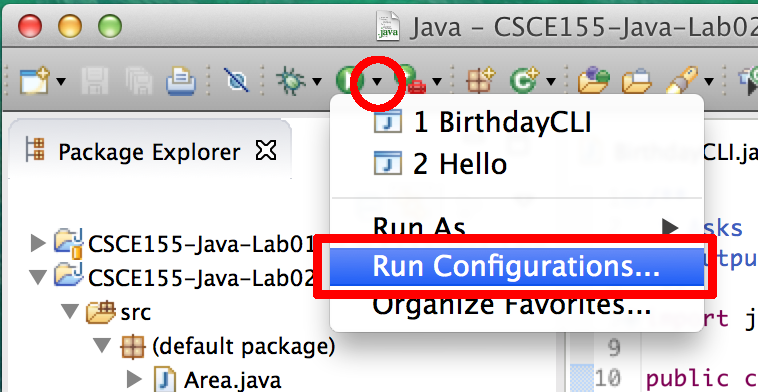
\includegraphics[scale=.45]{eclipseRunConfigurationMarkUp}
		\end{center}
	  \item Click the ``Arguments'' tab and enter the command 
		line arguments as follows: \mintinline{text}{James 1955 5 19}.
	  \item Click ``Apply'' then ``Run''
	\end{enumerate}
  \item Answer the questions on your worksheet.
\end{enumerate}

\subsection{Basic Data Types}

A variable is a name associated with a memory cell whose value can change. 
When variables are stored in memory, the computer has to have a way of 
knowing what type of data is stored in a given variable.  Data types identify 
the type of values stored in a memory location and operations that can be 
performed on those values.  A computer will not use the same amount of 
memory to store a single letter as it does to store a very large real number, 
and the values are not going to be interpreted the same way.  Therefore, 
different data types may have different sizes. The (incomplete) table in 
question 4 on the worksheet shows some basic data types with their 
sizes and ranges.  Size is represented in bytes.  A byte is a unit of storage 
capable of holding a single character.  A byte is usually considered equal 
to 8 bits.  A bit (short for binary digit), is the smallest unit of information in 
a computer--either a zero or a one.  Some basic data types can be either 
signed (either positive or negative) or unsigned (non-negative).

Java is a \emph{statically-typed} language; all variables must be declared 
by giving them a type and a name before they can be used.  Declarations 
can optionally be followed by an assignment in the same line.  Some 
examples:

\begin{minted}{java}
int a;
int b = 10;
int c, d = 5, e;
double x, pi = 3.14;
\end{minted}

For basic data types (called primitive data types), Java specifies exactly 
how many bytes each type takes and consequently defines a fixed range 
for each type.  A Java program has been provided, Ranges.java that 
demonstrates the size and range of each basic data type.

\subsubsection*{Instructions}

\begin{enumerate}
  \item Open the source file \mintinline{text}{Ranges.java} in your
	Eclipse project and run it.
  \item On the lab worksheet, complete all the size and range entries 
  	in the table with the values of the output of the program. 
\end{enumerate}

Note: Java also supports a primitive \mintinline{java}{boolean} type 
that can be assigned the value true or false.  Thus, there is no range.  
Conceptually, a \mintinline{java}{boolean} should only require one bit, 
however memory addressing would make this inefficient.  In practice, 
a \mintinline{java}{boolean} takes 32 bits if in the system stack, and 8
bits when used in arrays.
 
\subsection{Currency Conversion}

Write a program that will convert US Dollars to British Pounds and 
Japanese JPY.  10\% of the total amount of US Dollars will be taken 
as an exchange fee.  For the rest of the US Dollars, half will be 
changed to British Pounds and the other half to JPY.  Assume the 
exchange rate is: 1 US Dollar = 0.6 British Pound; 1 US Dollar = 
76.8 JPY.  The program should prompt the user to input the amount 
of US dollars then print an appropriate output.  An example run 
would look something like the following:

\begin{minted}{text}
Please input the total amount of US Dollars: 100.00
You get 27.00 British Pounds and 3456.00 Japanese JPY.
\end{minted}

\subsubsection*{Instructions}

\begin{enumerate}
  \item In Eclipse, create a new class named \mintinline{java}{Dollar}
  	by right-clicking your project and selecting New $\rightarrow$ class.
  \item Write your complete Java program in this source file.  Be sure to
  	place your code in a \mintinline{java}{main} method and 
	to choose appropriate data types for your variables
  \item Run your program and answer the questions on your worksheet.
\end{enumerate} 

\subsection{Mixed types}

A mixed-type expression is an expression with operands of different 
data types. When an assignment statement is executed, the expression 
on the right-hand-side is evaluated, and then the resulting value is 
placed into the variable on the left-hand-side.  For example:

\begin{minted}{java}
int x = (8 * 4) + (3 * .5);
\end{minted}

The data types of the operand affect the data type of the result.  This 
can lead to some initially unintuitive results.  When performing division 
between two integers, the result is necessarily an integer.  For example:

\begin{minted}{java}
int a = 10, b = 20, c;
c = a / b;
\end{minted}

In the code snippet above, the floating point result of \mintinline{c}{10 / 20} 
\emph{should} be \mintinline{c}{0.5}, but the actual value stored in the 
variable \mintinline{c}{c} is zero!  This is because the result of an operation 
of two integers is an integer: thus the decimal part of the result is truncated 
(dropped).  We could fix this by making at least one of the operands (and 
the resulting variable) a floating point variable through type-casting:

\begin{minted}{java}
int a = 10, b = 20;
double c;
c = (double) a / b;
\end{minted}

You have been given a Java program, \mintinline{text}{Area.java} that reads 
in the base and the height of a triangle and calculates the total area.

\begin{enumerate}
  \item Read through and understand the source code
  \item Compile and run your program to answer the remaining questions 
  	on your worksheet.
  \item Using the previous birthday programs as a reference, change the
  	area program to accept command line arguments instead of prompting
	for input.
\end{enumerate}  

\section{Handin/Grader Instructions}

\begin{enumerate}
  \item Hand in your \mintinline{text}{Area.java} source file by pointing your browser to:
  	\url{https://cse-apps.unl.edu/handin} and login with your CSE 
	login/password.
  \item Grade yourself by pointing your browser to 
  	\url{https://cse.unl.edu/~cse155h/grade/} (you may need to change the course
	in this URL depending on which course you are taking)
  \item Enter your cse login and password, select the appropriate assignment for 
  	this lab and click grade me.
  \item You will be displayed with both expected output and your program's output.  
	The formatting may differ slightly and that is not important.  As long as your 
	program successfully compiles, runs and outputs the same values, it is considered 
	correct.
\end{enumerate}  

Turn your completed worksheet in to the lab instructor.

\section{Advanced Activities (Optional)}

\begin{enumerate}
%  \item Modify the \mintinline{text}{Area.java} program to accept inputs from command 
%  	line arguments rather than prompting the user for input.  Note: command line inputs 
%	are always strings.  To convert to a particular data type, each primitive data type 
%	has a corresponding class that has several static functions for data type conversion.  
%	For example:
%
%\begin{minted}{java}	
%int a = Integer.parseInt(args[0]);
%double b = Double.parseDouble("3.14");
%\end{minted}

  \item Many applications require the use of numerical values greater than or with 
  	greater precision than what 32-bit signed integers and 64-bit floating point 
	numbers can represent.  It is typical to use a multi-precision library that offers 
	integers and floating point number types with arbitrary precision but with a 
	greater performance cost.  Java offers several classes as part of its Standard 
	Developer Kit (SDK): \mintinline{java}{BigInteger} (\url{http://docs.oracle.com/javase/8/docs/api/java/math/BigInteger.html}) 	and \mintinline{java}{BigDecimal} (\url{http://docs.oracle.com/javase/8/docs/api/java/math/BigDecimal.html}).  
	Read the provided documentation and modify your program to use these 
	types instead so that US National Debt can be represented and correctly 
	converted to Yen. 
\end{enumerate}

\end{document}
